\documentclass{beamer}
\usetheme{Copenhagen}
\usecolortheme{beaver} 

\title{Python in a physics lab}
\author{Gergely Imreh}
\date{PyCon Taiwan \\ \today}


\begin{document}

\maketitle

\section{Lab overview}

\begin{frame}{A sample slide}


\end{frame}

\section{Experiment X}

\subsection{Preparation}

\begin{frame}{Theory}

\begin{itemize}
	\item Numpy - Numerical Python
	\item SciPy - Scientific Python
	\item SymPy - Symbolic Math
	\item QuTIP$^2$ - Quantum Toolkit
	\item multiprocessing
\end{itemize}

\begin{figure}[ht]
	
\includegraphics[width=8cm]{numerical.png}
\end{figure}

\end{frame}


\subsection{Talking to instruments}

\begin{frame}[fragile]

\textbf{GPIB: General Purpose Interface Bus}

\begin{verbatim}
import visa
oscilloscope = visa.instrument("GPIB::12")
print oscilloscope.ask("*IDN?")
\end{verbatim}

\begin{figure}[ht]
	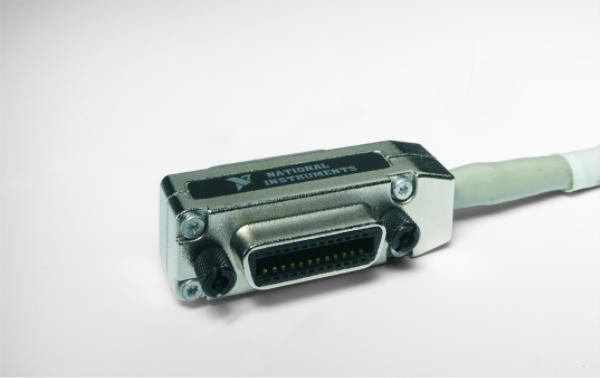
\includegraphics[width=8cm]{gpib1.JPG}
\end{figure}

\end{frame}


\subsection{Interface}

\begin{frame}{A sample slide}


\end{frame}

\subsection{Analysis}

\begin{frame}{A sample slide}


\end{frame}

\section{Verdict}

\begin{frame}{A sample slide}


\end{frame}

\begin{frame}[fragile]


\textbf{imrehg@gmail.com}

https://gergely.imreh.net

https://github.com/imrehg

\begin{figure}[ht]
	
\includegraphics[width=3cm]{Oxford_Logo.png}
	
\includegraphics[width=3cm]{Sinica_Logo.png}
	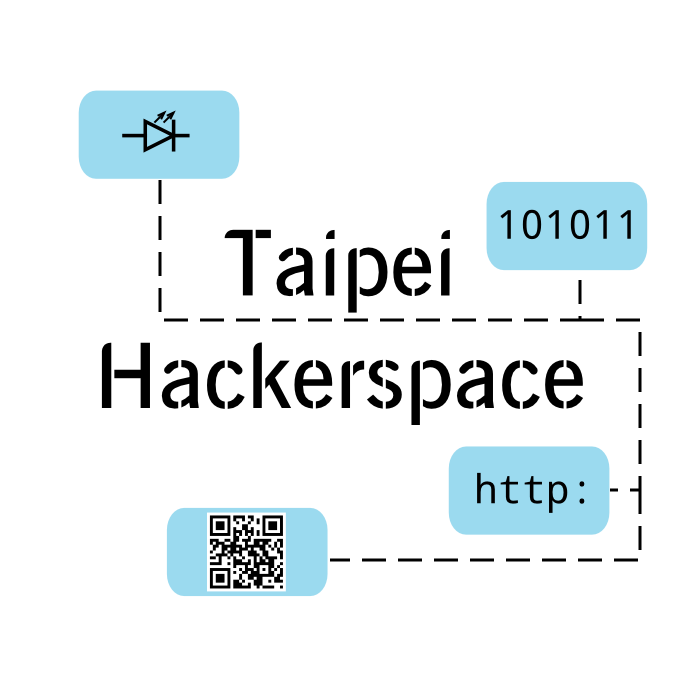
\includegraphics[width=3cm]{Hackerspace_Logo.png}
\end{figure}


\end{frame}


\end{document}